\subsection{Bifurcação}

%--------------------

\begin{frame}
\vspace{5pt}
\frametitle{Família Quadrática: \subsecname}
\begin{columns}
\column{\dimexpr\paperwidth-15pt}

Seja $f_\lambda$ uma família parametrizada de funções no parâmetro $\lambda$ de modo que a função
$$G(x, \lambda) = f_\lambda(x),$$
definida num aberto de $\RR^2$, seja de classe $\class^\infty$ nas variáveis $x$ e $\lambda$.

\begin{definition}
Dizemos que a família $f_\lambda$ sofre uma bifurcação em $\lambda_0$ se existe $\varepsilon > 0$ com a seguinte propriedade: se $\lambda_1 \in (\lambda_0 - \varepsilon, \lambda_0)$ e $\lambda_2 \in (\lambda_0, \lambda_0 + \varepsilon)$, então $f_{\lambda_1}$ e $f_{\lambda_2}$ não são topologicamente conjugadas.
\end{definition}

\end{columns}
\end{frame}

%--------------------

\begin{frame}
\vspace{5pt}
\frametitle{Família Quadrática: \subsecname}
\begin{columns}
\column{\dimexpr\paperwidth-15pt}

\begin{block}{Exemplo}
A família $E_\lambda$ de funções dadas por $E_\lambda(x) = e^{x + \lambda}$ sofre uma bifurcação em $\lambda_0 = -1$.

\begin{figure}[!htb]
\centering
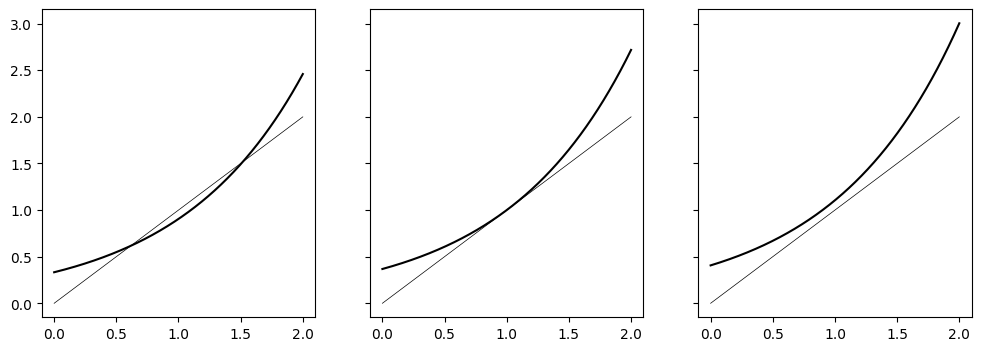
\includegraphics[scale=0.4]{images/e_lambda.png}
\caption{Gráficos de $E_\lambda$ numa vizinhança de $1$ para $\lambda = -1.1$, $\lambda = -1$ e $\lambda = -0.9$.}
\label{e_lambda}
\end{figure}

Uma bifurcação com essas características é chamada de bifurcação tangente.
\end{block}

\end{columns}
\end{frame}

%--------------------

\begin{frame}
\vspace{5pt}
\frametitle{Família Quadrática: \subsecname}
\begin{columns}
\column{\dimexpr\paperwidth-15pt}

\begin{block}{Exemplo}
A família quadrática sofre uma bifurcação em $\mu_0 = 3$.

\begin{figure}[!htb]
\centering
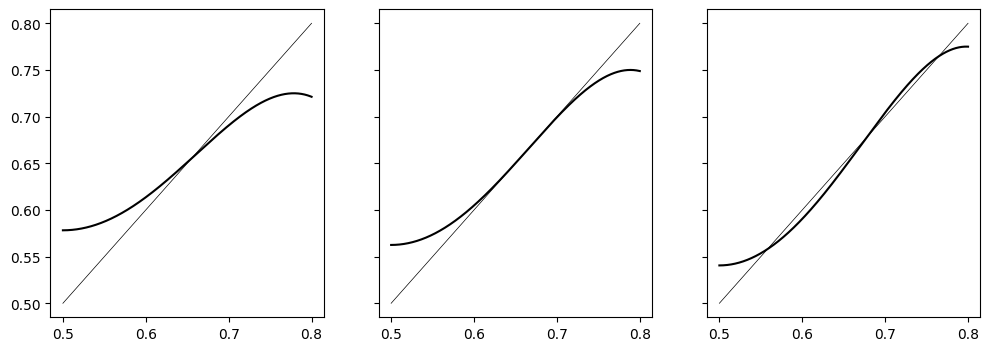
\includegraphics[scale=0.4]{images/h_3^2.png}
\caption{Gráficos de $h^2$ numa vizinhança de $p_\mu$ para $\mu = 2.9$, $\mu = 3$ e $\mu = 3.1$.}
\label{h_mu^2}
\end{figure}

Uma bifurcação com essas características é chamada de bifurcação com duplicação de período.
\end{block}

\end{columns}
\end{frame}

%--------------------

\begin{frame}
\vspace{5pt}
\frametitle{Família Quadrática: \subsecname}
\begin{columns}
\column{\dimexpr\paperwidth-15pt}

Observe, nos exemplos, que as bifurcações ocorreram quando a derivada em módulo no ponto fixo se tornou igual à $1$. O teorema a seguir mostra que isso não é coincidência.

\begin{theorem}
Seja $f_\lambda$ uma família parametrizada de funções.
Suponha que
\begin{enumerate}
\item $f_{\lambda_0}(x_0) = x_0$,
\item $f'_{\lambda_0}(x_0) \neq 1$. 
\end{enumerate}
Então existem vizinhanças $I$ e $J$ de $\lambda_0$ e $x_0$, respectivamente, e uma função $p: I \to J$ de classe $\class^\infty$ tais que
\begin{enumerate}
\item $p(\lambda_0) = x_0$, 
\item $f_\lambda(p(\lambda)) = p(\lambda)$ para todo $\lambda \in I$.
\end{enumerate}
Além disso, $f_\lambda$ não possui outros pontos fixos em $J$.
\end{theorem}

\end{columns}
\end{frame}

%--------------------

\begin{frame}
\vspace{5pt}
\frametitle{Família Quadrática: \subsecname}
\begin{columns}
\column{\dimexpr\paperwidth-15pt}

Vamos estudar com mais detalhes a bifurcação com duplicação de período que ocorre na família quadrática.

Se $\mu > 2$, então existe $p_\mu' < p_\mu$ tal que $h(p_\mu') = p_\mu$.
Observe, na figura abaixo, os gráficos de $h^2$ para alguns valores de $\mu$, juntamente com um quadrado de vértices $(p_\mu', p_\mu)$, $(p_\mu, p_\mu)$, $(p_\mu, p_\mu')$ e $(p_\mu', p_\mu')$.

\begin{figure}[!htb]
\centering
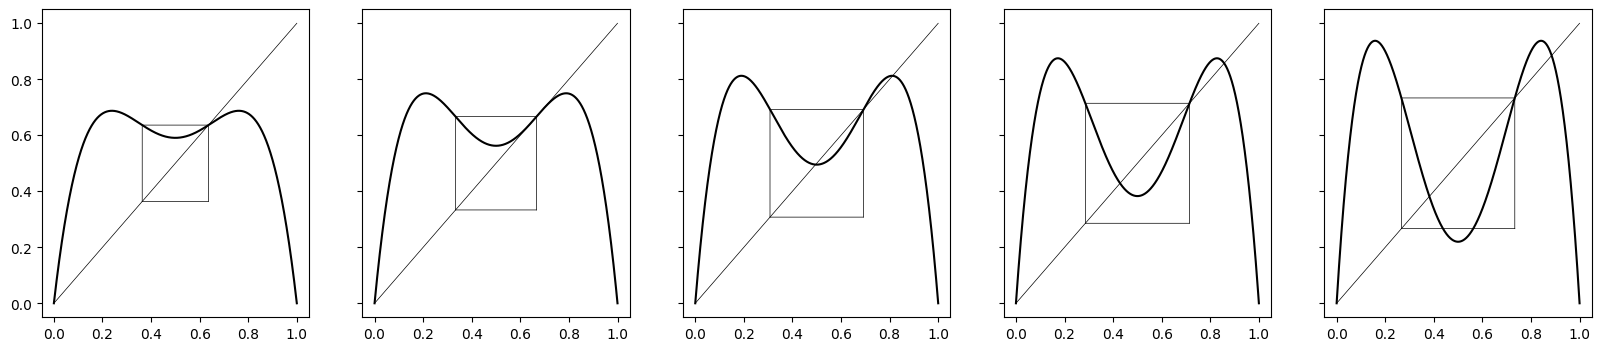
\includegraphics[scale=0.375]{images/h^2withboxes.png}
\caption{Gráficos de $h^2$ para $\mu = 2.75$, $\mu = 3$, $\mu = 3.25$, $\mu = 3.5$ e $\mu = 3.75$.}
\label{h^2-and-boxes}
\end{figure}

\end{columns}
\end{frame}

%--------------------

\begin{frame}
\vspace{5pt}
\frametitle{Família Quadrática: \subsecname}
\begin{columns}
\column{\dimexpr\paperwidth-15pt}

Restringindo o gráfico de $h^2$ ao quadrado e rotacionando em $\pi$ radianos, vemos que ele se assemelha ao gráfico da própria $h$ no intervalo $[0, 1]$ para um valor de $\mu$ diferente.

Considere a função $L: [p_\mu', p_\mu] \to [0, 1]$ linear tal que $L(p_\mu') = 1$ e $L(p_\mu) = 0$. Definimos a renormalização de $h$ como a função $Rh: [0, 1] \to [0, 1]$ dada por
$$Rh(x) = L \circ h^2 \circ L^{-1}(x).$$

\begin{figure}[!htb]
\centering
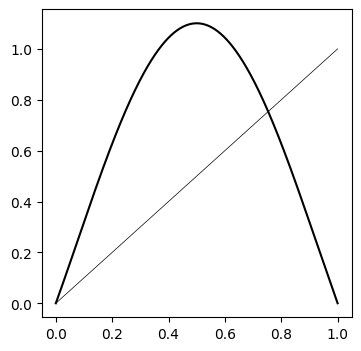
\includegraphics[scale=0.4]{images/renormalization.png}
\caption{Gráfico de $Rh$ para $\mu = 3.75$.}
\label{renormalization}
\end{figure}

\end{columns}
\end{frame}

%--------------------

\begin{frame}
\vspace{5pt}
\frametitle{Família Quadrática: \subsecname}
\begin{columns}
\column{\dimexpr\paperwidth-15pt}

Observe que cada ponto fixo de $Rh$ está relacionado com um ponto periódico de $h$ de período $2$. Além disso, o gráfico de $Rh$ não está contido em $[0, 1]$ para algum $\mu < 4$.

Desse modo, esperamos que $Rh$ sofra uma bifurcação com duplicação de período conforme o parâmetro cresce e, de maneira análoga, que $h^2$ sofra uma bifurcação com duplicação de período. Continuando esse processo, temos uma sucessão de bifurcações com duplicação de período na família quadrática.

\end{columns}
\end{frame}

%--------------------

\begin{frame}
\vspace{5pt}
\frametitle{Família Quadrática: \subsecname}
\begin{columns}
\column{\dimexpr\paperwidth-15pt}

O computador nos permite observar esse fato experimentalmente.
Para isso, vamos computar o digrama de órbita do ponto crítico da família quadrática para $\mu > 2$.



\end{columns}
\end{frame}

%--------------------

\begin{frame}
\vspace{5pt}
\frametitle{Família Quadrática: \subsecname}
\begin{columns}
\column{\dimexpr\paperwidth-15pt}

\begin{figure}[!htb]
\centering
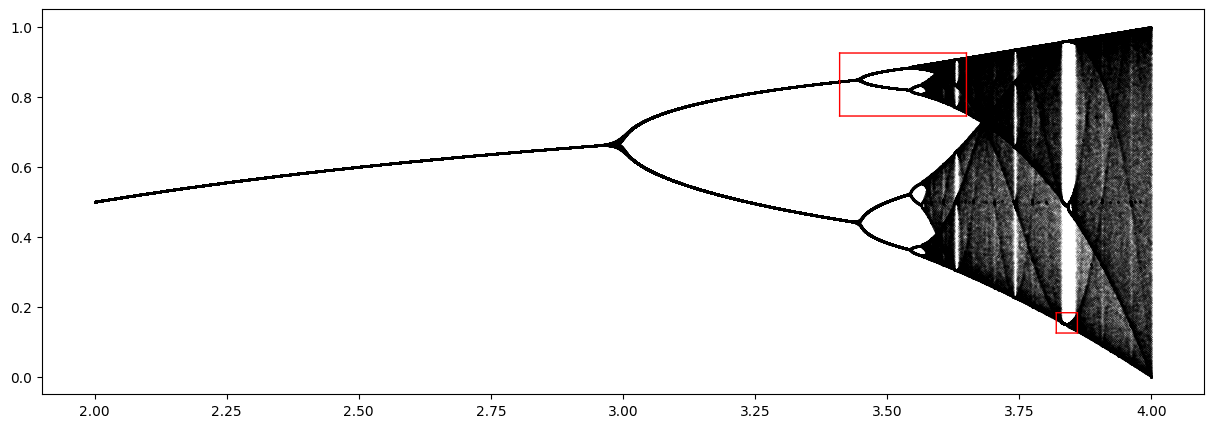
\includegraphics[scale=0.4]{images/period-doubling-and-zoom1.png}
\caption{Diagrama de órbita de $h$ para $\mu \in [2, 4]$.}
\label{period-doubling}
\end{figure}

\end{columns}
\end{frame}

%--------------------

\begin{frame}
\vspace{5pt}
\frametitle{Família Quadrática: \subsecname}
\begin{columns}
\column{\dimexpr\paperwidth-15pt}

\begin{figure}[H]
\centering
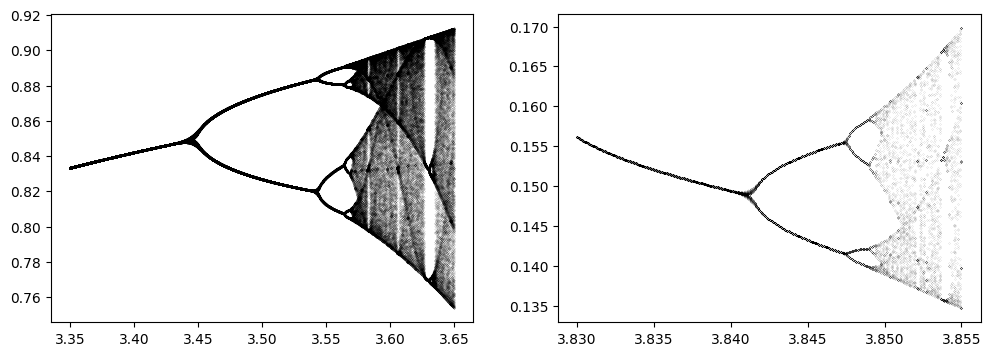
\includegraphics[scale=0.4]{images/period-doubling-and-zoom2.png}
\caption{Ampliação das regiões retangulares marcadas na Figura \ref{period-doubling}.}
\label{period-doubling1}
\end{figure}

\end{columns}
\end{frame}
